\section*{Appendix}
\begin{frame}[noframenumbering,label=CFG]
\frametitle{Control-flow graph (CFG)}
%
\emph{Basic blocks} sequence of consecutive statements\\
\emph{Edges} control flow (jumps or fall-through)\\
\vskip5mm
\hfill
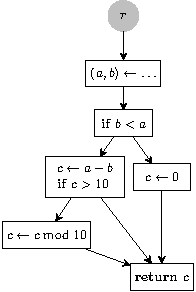
\includegraphics[valign=t,scale=0.9]{cfg-nonssa}\hfill
% 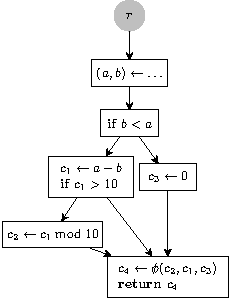
\includegraphics[valign=t,scale=0.9]{cfg-ssa}\hfill
\begin{minipage}[t]{0.25\textwidth}
\footnotesize
\textperiodcentered$(a,b)\gets \ldots$\\
\textperiodcentered$\textbf{if } b<a\textbf{ then}$\\
\textperiodcentered\hspace{1em}$c\gets a-b$\\
\textperiodcentered\hspace{1em}$\textbf{if } c>10\textbf{ then}$\\
\textperiodcentered\hspace{2em}$c \gets c \bmod 10$\\
\textperiodcentered\hspace{1em}$\textbf{endif}$\\
\textperiodcentered\textbf{else}\\
\textperiodcentered\hspace{1em}$c\gets 0$\\
\textperiodcentered$\textbf{endif}$\\
\textperiodcentered$\textbf{return } c$
\bigskip
\end{minipage}\hfill\strut
\vfill\hfill\hyperlink{inf-semantics<2>}{\beamerreturnbutton{Back}}\vskip1cm
\end{frame}

\begin{frame}[noframenumbering,label=DomTree]
\frametitle{Tree-shape. Dominance}

\begin{minipage}{0.48\textwidth}
    \emph{Dominance relation}
    \begin{itemize}
    \item a single entry node $r$.
    \item each node reachable from~$r$.
    \item $a$ dominates $b$ if every path from $r$ to $b$ contains $a$.
    \end{itemize}
    
    \uncover<3>{
      \emph{Properties}
      \begin{itemize} 
      \item The dominance relation induces a \alert{tree}. 
      \end{itemize}
    }
\end{minipage}
\hfill
\begin{minipage}{0.5\textwidth}
\only<1>{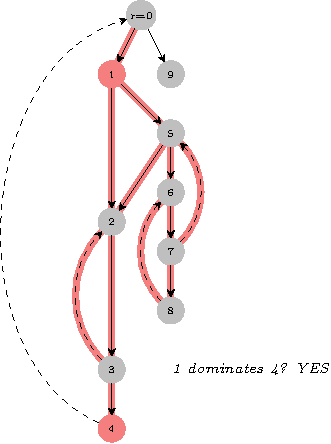
\includegraphics[scale=0.8]{dominance-1}}%
\only<2>{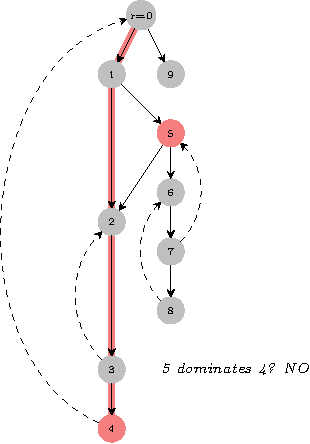
\includegraphics[scale=0.8]{dominance-2}}%
\only<3>{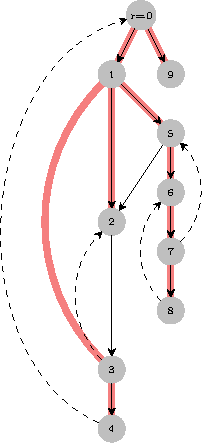
\includegraphics[scale=0.8]{dominance-3}}%
\end{minipage}
\end{frame}

\begin{frame}[noframenumbering,label=strictSSA]
  \frametitle{Static Single Assignment with dominance property}
  \begin{columns}
    \column{0.6\textwidth}
    \begin{block}{Strict code}
      Every path from $r$ to a \emph{use} traverses a definition
    \end{block}
    \begin{block}{Strict SSA}
      \begin{itemize}
      \item \alert{SSA}: only \emph{one} definition \emph{textually} per variable
      \item \alert{Strict}: the definition dominates all uses
      \end{itemize}
    \end{block}
    \hfill
    \column{0.35\textwidth}
    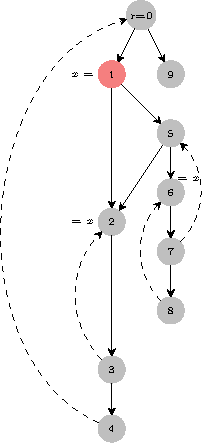
\includegraphics[scale=0.8]{strictSSA}
  \end{columns}
\end{frame}

\begin{frame}[noframenumbering,label=chordal]
  \frametitle{Liveness: sub-tree of a tree}
  \begin{columns}
    \column{0.6\textwidth}
      \begin{block}{The live-range of an SSA variable is}
        the set of program points\\ \alert{between the definition and a use}\\
        \footnotesize (\emph{without going through the definition again})
      \end{block}
    \begin{itemize}
      \item<2> the definition dominates the entire live-range
      \item<2> the live-range is a \green{sub-tree} of the \red{dominance-tree}
    \end{itemize}
    \column{0.35\textwidth}
    \only<1>{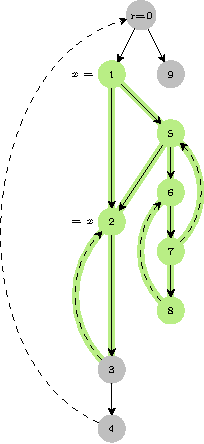
\includegraphics[scale=0.8]{subtree-1.pdf}}%
    \only<2>{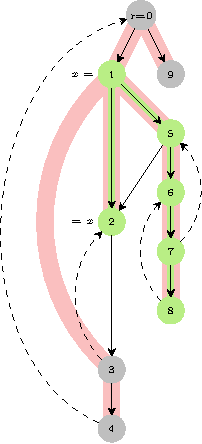
\includegraphics[scale=0.8]{subtree-2.pdf}}%
  \end{columns}
\end{frame}

\begin{frame}[noframenumbering,label=spilltest]
  \frametitle{``Spilling easier on a BB than on a general CFG''\hyperlink{allocation}{\beamerreturnbutton{}}}
    \begin{columns}
    \column{0.3\textwidth}{%BB large
      \begin{center}
	\blue{Basic block}\\
	\only<1>{\includegraphics[height=5cm]{code_BB-1.fig}}%
	\only<2>{\includegraphics[height=5cm]{code_BB-2.fig}}%
	\only<3>{\includegraphics[height=5cm]{code_BB-3.fig}}%
	\only<4>{\includegraphics[height=5cm]{code_BB-4.fig}}%
	\only<5>{\includegraphics[height=5cm]{code_BB-5.fig}}%
	\only<6>{\includegraphics[height=5cm]{code_BB-6.fig}}%
	\only<7>{\includegraphics[height=5cm]{code_BB-7.fig}}%
	\only<8>{\includegraphics[height=5cm]{code_BB-8.fig}}%
	\only<9>{\includegraphics[height=5cm]{code_BB-9.fig}}%
	\only<10>{\includegraphics[height=5cm]{code_BB-10.fig}}%
	\only<11>{\includegraphics[height=5cm]{code_BB-11.fig}}%
	\only<12>{\includegraphics[height=5cm]{code_BB-12.fig}}%
	\only<13>{\includegraphics[height=5cm]{code_BB-13.fig}}%
	\only<14>{\includegraphics[height=5cm]{code_BB-14.fig}}%
	\begin{block}{}
	  \begin{itemize}
	  \item $\textsf{MAXLIVE}\leq r$
	  \item Linear scan
	  \end{itemize}
	\end{block}
      \end{center}
    }
    \column{0.3\textwidth}{%SSA small
      \begin{center}
	\blue{SSA code}\\
	\includegraphics[height=2.5cm]{code_SSA-1.fig}%
      \end{center}
    }
    \column{0.3\textwidth}{%CFG small
      \begin{center}
	\blue{General CFG}\\
	\includegraphics[height=2.5cm]{code_CFG-1.fig}    
      \end{center}
    }
    \end{columns}
\end{frame}
 
%CFG
\begin{frame}[noframenumbering]
  \frametitle{``Spilling easier on a BB than on a general CFG''}
  \begin{columns}
    \column{0.15\textwidth}{%BB
      \begin{center}
	\blue{BB}\\
	\includegraphics[height=2.5cm]{code_BB-8.fig}
      \end{center}
    }
    \column{0.15\textwidth}{%SSA small
       \begin{center}
	 \blue{SSA}\\
	 \includegraphics[height=2.5cm]{code_SSA-1.fig}%
       \end{center}
    }
    \column{0.45\textwidth}{%CFG
      \begin{center}
	\blue{General control flow graph}\\
	\includegraphics[height=5cm]{code_CFG_static.fig}    
	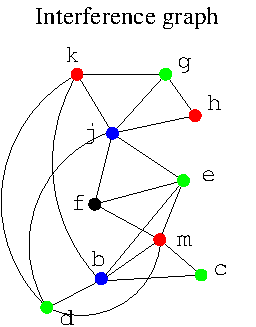
\includegraphics[height=3cm]{IntGraph-stuck.fig}  
	\begin{alertblock}{}
	  \begin{itemize}
	  \item Coloring test
	  \item Greedy coloring
	  \end{itemize}
	\end{alertblock}
      \end{center}
   }%
  \end{columns}
\end{frame}

%SSA
\begin{frame}[noframenumbering]
  \frametitle{``Under SSA: the dominance tree''\hyperlink{allocation}{\beamerreturnbutton{}}}
    \begin{columns}
    \column{0.15\textwidth}{%
      \begin{center}
	\blue{BB}\\
	\includegraphics[height=2.5cm]{code_BB-8.fig}
      \end{center}
    }
    \column{0.55\textwidth}{%
      \begin{center}
	\blue{Static single assignment form}\\
	\only<1>{\includegraphics[height=5cm]{code_SSA-1.fig}}%
	\only<2>{\includegraphics[height=5cm]{code_SSA-2.fig}}%
	\only<3>{\includegraphics[height=5cm]{code_SSA-3.fig}}%
	\only<4>{\includegraphics[height=5cm]{code_SSA-4.fig}}%
	\only<5>{\includegraphics[height=5cm]{code_SSA-5.fig}}%
	\only<6>{\includegraphics[height=5cm]{code_SSA-6.fig}}%
	\only<7>{\includegraphics[height=5cm]{code_SSA-7.fig}}%
	\only<8>{\includegraphics[height=5cm]{code_SSA-8.fig}}%
	\only<9>{\includegraphics[height=5cm]{code_SSA-9.fig}}%
	\only<10>{\includegraphics[height=5cm]{code_SSA-10.fig}}%
	\only<11>{\includegraphics[height=5cm]{code_SSA-11.fig}}%
	\only<12>{\includegraphics[height=5cm]{code_SSA-12.fig}}%
	\only<13>{\includegraphics[height=5cm]{code_SSA-13.fig}}%
	\only<14>{\includegraphics[height=5cm]{code_SSA-14.fig}}%
	\begin{block}{}
	  \begin{itemize}
	  \item $\textsf{MAXLIVE}\leq r$
	  \item Tree scan
	  \end{itemize}
	\end{block}
      \end{center}
    }%
    \column{0.3\textwidth}{%
      \begin{center}
      \blue{CFG}\\
      \includegraphics[height=2.5cm]{code_CFG_static.fig}    
      \includegraphics[height=1.5cm]{IntGraph.fig}  
      \end{center}
    }     
  \end{columns}
\end{frame}

\begin{frame}[noframenumbering]
  \frametitle{``Under SSA: the dominance tree''\hyperlink{allocation}{\beamerreturnbutton{}}}
    \begin{columns}
    \column{0.28\textwidth}{%BB
      \blue{Basic block}\\
      \includegraphics[height=3.5cm]{code_BB-8.fig}
      \begin{block}{}
	\begin{itemize}
	  \item $\textsf{MAXLIVE}\leq r$
	  \item Linear scan
	\end{itemize}
      \end{block}
    }
    \column{0.28\textwidth}{%SSA
      \blue{SSA form}\\
      \includegraphics[height=3.5cm]{code_SSA-8.fig}%
    \begin{block}{}
	 \begin{itemize}
	 \item $\textsf{MAXLIVE}\leq r$
	 \item Tree scan
	 \end{itemize}
      \end{block}
    }%
    \column{0.35\textwidth}{%CFG
      \blue{General CFG}\\
      \includegraphics[height=3.5cm]{code_CFG_static.fig}    
      \includegraphics[height=2cm]{IntGraph.fig}  
      \begin{alertblock}{}
	\begin{itemize}
	\item Coloring test
	\item Greedy coloring
	\end{itemize}
      \end{alertblock}
    }     
  \end{columns}
\end{frame}
